
\documentclass[a4paper,12pt]{article} 
\usepackage[top = 2.5cm, bottom = 2.5cm, left = 2.5cm, right = 2.5cm]{geometry} 

\usepackage[T1]{fontenc}
\usepackage{hyperref}
\usepackage[utf8]{inputenc}
\usepackage{algorithm,algpseudocode}
\usepackage{amsthm}
\usepackage{amsmath}
\usepackage{xcolor}
\newtheorem{proposition}{Proposition}

\usepackage{tikz}
\usepackage{pgfplots}
\usepackage{multirow} 
\usepackage{booktabs}
\usepackage{graphicx} 
\usepackage{listings}
\lstset{language=C++,
	numbers=none,
	showspaces=false,
	showstringspaces=false,
	basicstyle=\small}

\usepackage{setspace}
\setlength{\parindent}{0in}

\usepackage{float}

\usepackage{fancyhdr}
\pagestyle{fancy}
\fancyhf{}

\usepackage{mathtools}
\DeclarePairedDelimiter\ceil{\lceil}{\rceil}
\DeclarePairedDelimiter\floor{\lfloor}{\rfloor}
\newcommand{\bigO}{\mathcal{O}}
\lhead{\footnotesize The Sieve of Eratosthenes}
\rhead{\footnotesize Michael Markl} 


\cfoot{\footnotesize \thepage} 


\newcommand{\todo}[1]{{\color{red}#1}}

\DeclareMathOperator{\currPrime}{currPrime}
\DeclareMathOperator{\currCoord}{currCoord}
\DeclareMathOperator{\lastCoord}{lastCoord}
\DeclareMathOperator{\crosses}{crosses}
\renewcommand{\lstlistingname}{Program}
\newcommand{\algorithmautorefname}{Algorithm}
\newcommand{\propositionautorefname}{Proposition}


\begin{document}

\thispagestyle{empty}

\begin{tabular}{p{15.5cm}} %
{\large \bf Parallel Algorithms} \\
University of Utrecht \\ Fall 2020  \\ Rob H. Bisseling\\
\hline
\\
\end{tabular}

\vspace*{0.3cm}
\begin{center}
	{\Large \bf The Sieve of Eratosthenes}
	\vspace{2mm}
	
	{\bf Michael Markl}
\end{center}  
\vspace{0.4cm}

\section{An ancient primality test}

Prime numbers play a central role for example in modern encryption algorithms.
Most encryption algorithms need prime numbers with about 1,000 digits as a secret key.
Hence, many algorithms chose some number randomly and then check with so-called primality tests, whether this number is a prime number and therefore suitable for using as an encryption key.

One such primality test, which was already invented by the ancient greeks, is called the Sieve of Eratosthenes.
This algorithm not only checks for a given number whether it is prime, but it even finds all prime numbers up to that number.
Given the number $n$ the procedure starts with a list of the numbers from $2$ to $n$.
It starts with $2$ and cross out all larger multiples of $2$.
Then it continues with the next number which is not crossed out -- in the second iteration the number $3$ -- and crosses out all larger multiples of it.
This procedure is repeated until the whole list is worked through.
Then all numbers that are not crossed out in the end are exactly all prime numbers up to the number $n$.

For generating all prime numbers up to $n$ it even suffices to iterate this procedure until the number~$\floor{\sqrt{n}}$: If we assume, that $x\leq n$ is not a prime number, we find numbers $a,b\in\{2, \dots, x\}$ with $x=a\cdot b$.
If $a$ or $b$ is smaller than or equal to $\floor{\sqrt{n}}$ then $x$ would be crossed out after reaching $\floor{\sqrt{n}}$.
Otherwise, $a$ and $b$ are strictly larger than $\floor{\sqrt{n}}$ which implies that $a$ and $b$ are strictly larger than $\sqrt{n}$ and hence $x = a\cdot b > \sqrt{n}^2 = n \geq x$ forms a contradiction.

Even faster: Once we choose to erase all larger multiples of some number, we can choose to start with its square, as all other multiples -- if existent -- have already been taken care of when crossing out multiples of smaller numbers.

This very simple algorithm is implemented in~\autoref{prg:seq_sieve} using the programming language C++.
It initalises an array of size $n-1$ for the numbers $2,\dots, n$ with the value $\mathbf{false}$.
We now interpret $\crosses[i] == \mathbf{true}$ as the number $i+2$ being crossed out, and sequentially go through all numbers up to $n$ and cross out larger multiples of primes as explained above.
Operations involving the variable $\mathrm{numberOps}$ in~\autoref{prg:seq_sieve} are only used for numerically evaluating the cost of the algorithm, which we will come to after analyzing the asymptotic cost.

\begin{proposition}\label{prop:seq_sieve}
	The sequential implementation in~\autoref{prg:seq_sieve} has cost $\bigO(n \log \log n)$.
\end{proposition}
\begin{proof}
	We may assume that computing the square root, and that the allocation of memory has constant cost.
	Then the initialisation of the variables takes $\bigO(n)$ steps.
	The outer loop has at most $\floor{\sqrt{n}}$ iterations and for each iteration, if a prime number $p$ was found, it takes another $\floor{n / p}$ to cross out all larger multiples of $p$.
	Using that the probability that a natural number $x$ is a prime number is about $1/\ln x$, we can bound the overall asymptotic expected cost of the outer loop by
	\[
		\sqrt n + \sum_{\substack{p = 2 \\ \text{$p$ is prime}}}^{\floor{\sqrt{n}}} \frac{n}{p} \leq \sqrt{n} + n \sum_{k = 2}^n \frac{1}{k \ln k}
	\]
	Approximating $\sum_{k=2}^n 1/(k\ln k)$ by the integral $\int_2^n 1 / (x \ln x) \,\mathrm{d}x$ yields the asymptotic bound
	\[
		n \int_2^n \frac{1}{x \ln x}\, \mathrm{d}x = n \left[ \ln(\ln(x)) \right]_2^n = \bigO(n\log\log n ).
	\]
	As the second only iterates through all numbers and collects those numbers that are not crossed out, this proves the proposition.
\end{proof}


\begin{figure}
	\caption{Numerical analysis of the cost of the sequential Sieve of Eratosthenes}
	\centering
	\label{fig:seq_sieve}
	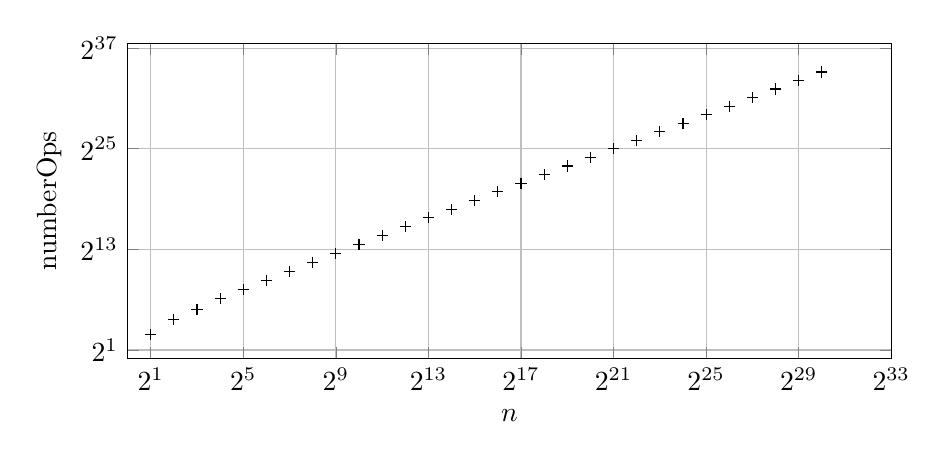
\begin{tikzpicture}
	\begin{loglogaxis}[
	scale only axis,
	width=0.8\textwidth,
	xmin=1,
	ymin=1,
	log basis x=2,
	log basis y=2,
	height=4cm,
	xlabel=$n$, 
	ylabel=$\mathrm{numberOps}$,
	grid=major]
	\addplot[only marks, mark=+] coordinates {
		(2,7)
		(4,25)
		(8,55)
		(16,136)
		(32,294)
		(64,643)
		(128,1352)
		(256,2857)
		(512,5985)
		(1024,12460)
		(2048,25799)
		(4096,53321)
		(8192,109899)
		(16384,225963)
		(32768,463232)
		(65536,948197)
		(131072,1937555)
		(262144,3953140)
		(524288,8054276)
		(1048576,16390356)
		(2097152,33320258)
		(4194304,67670963)
		(8388608,137305652)
		(16777216,278369997)
		(33554432,563949620)
		(67108864,1141764130)
		(134217728,2310197689)
		(268435456,4671690591)
		(536870912,9442275539)
		(1073741824,19075519083)
	};
	\end{loglogaxis}
	\end{tikzpicture}
	
	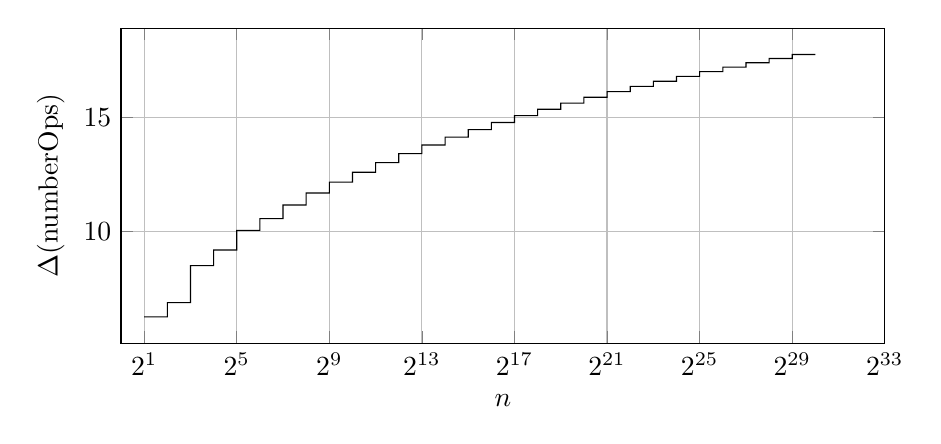
\begin{tikzpicture}
	\begin{semilogxaxis}[
	scale only axis,
	width=0.8\textwidth,
	xmin=1,
	log basis x=2,
	log basis y=2,
	height=4cm,
	xlabel=$n$, 
	ylabel=$\Delta(\mathrm{numberOps})$,
	grid=major]
	\addplot[] coordinates {
		(2.001000,6.250000)
		(4,6.250000)
		(4.001000,6.875000)
		(8,6.875000)
		(8.001000,8.500000)
		(16,8.500000)
		(16.001000,9.187500)
		(32,9.187500)
		(32.001000,10.046875)
		(64,10.046875)
		(64.001000,10.562500)
		(128,10.562500)
		(128.001000,11.160156)
		(256,11.160156)
		(256.001000,11.689453)
		(512,11.689453)
		(512.001000,12.167969)
		(1024,12.167969)
		(1024.001000,12.597168)
		(2048,12.597168)
		(2048.001000,13.017822)
		(4096,13.017822)
		(4096.001000,13.415405)
		(8192,13.415405)
		(8192.001000,13.791687)
		(16384,13.791687)
		(16384.001000,14.136719)
		(32768,14.136719)
		(32768.001000,14.468338)
		(65536,14.468338)
		(65536.001000,14.782372)
		(131072,14.782372)
		(131072.001000,15.080032)
		(262144,15.080032)
		(262144.001000,15.362312)
		(524288,15.362312)
		(524288.001000,15.631062)
		(1048576,15.631062)
		(1048576.001000,15.888337)
		(2097152,15.888337)
		(2097152.001000,16.134015)
		(4194304,16.134015)
		(4194304.001000,16.368109)
		(8388608,16.368109)
		(8388608.001000,16.592145)
		(16777216,16.592145)
		(16777216.001000,16.807008)
		(33554432,16.807008)
		(33554432.001000,17.013611)
		(67108864,17.013611)
		(67108864.001000,17.212314)
		(134217728,17.212314)
		(134217728.001000,17.403404)
		(268435456,17.403404)
		(268435456.001000,17.587609)
		(536870912,17.587609)
		(536870912.001000,17.765462)
		(1073741824,17.765462)
	};
	\end{semilogxaxis}
	\end{tikzpicture}
	
\end{figure}


Now, for the numerical analysis we may assume that summations, mulitplications and taking square roots as well as evaluating comparisons takes one operation.
Then the variable $\mathrm{numberOps}$ counts the number of operations used in~\autoref{prg:seq_sieve}.
The first graph in~\autoref{fig:seq_sieve} shows the number of operations used for a given number $n$.
As expected, the factor of $\log\log n$ does not play any role at first glance as the plot given by the simulation strongly resembles a linear plot.
But having a closer look at the numbers, we can actually find out, that the number of operations is not linear:
Using the difference quotient for intervals $I\coloneqq [2^k, 2^{k+1}]$ defined as
\[\Delta(\mathrm{numberOps})_I\coloneqq \frac{\mathrm{numberOps}(2^{k+1}) - \mathrm{numberOps}(2^{k})}{2^k},\]
we can obtain more fine-grain statements about the growth-rate of the number of operations.
In the second graph of~\autoref{fig:seq_sieve} this series of difference quotients is displayed which shows that the growth is increasing and hence the number of operations is not linear just like in~\autoref{prop:seq_sieve}.
In fact, it supports the statement that the bound in~\autoref{prop:seq_sieve} is asymptotically tight, as the graph resembles the logarithm where the $x$-axis itself is logarithmic.
Hence $\Delta(\mathrm{numberOps})$ resembles $\log\log n$.


\section{A parallel algorithm of the Sieve of Eratosthenes}

When coming up with an idea to parallelise this algorithm, one needs to consider several questions:
What kind of work can be easily parallelised?
How should the numbers be distributed over the processors and what are the implications for designing the parallel algorithm?

First, let us discuss which parts of the algorithm can be worked on simultaneously.
The algorithm roughly consists of two repeated steps:
\begin{enumerate}
	\item Search for the next prime, i.e. the next number that is not crossed out.
	\item Cross out all larger multiples of the selected number.
\end{enumerate}
Trying to parallelise the first step would lead to multiple processors looking for a reasonable number they can use to erase all larger multiples of.
In doing so, it is inevitable that processors might choose some number that turns out not to be prime.
This does not lead to wrong calculations if no number is skipped, because crossing out all larger multiples of a composite number will of course not cross out any prime, but it introduces duplicate work:
If a prime dividing the composite number is chosen by a processor, then all the multiples of the composite number will be checked again.

Hence, the better idea may be to parallelise the second step.
In fact, once a number has been chosen and is known to every processor, each processor can cross out all larger multiples of that number located in its share of all numbers up to $n$.
The next arising question is: Who is responsible for deciding on the multiples of which number to work on next?
It should be a processor which is able to tell the next number that is not crossed out.
Therefore, it makes sense to arrange the numbers in blocks of equal size and start with the first processor to be the so-called \emph{coordinator}, as we know for sure, that for the next couple of iterations the next number, which is not crossed out, will be contained in its block.
Once the processor reaches the end of its block it can transfer the responsibility of coordination on to the next processor.

A benefit of this approach is, that communication between processors is very limited:
In each iteration, the coordinator only has to broadcast either the selected number or the new coordinator.

As we only have to process numbers up to $\sqrt{n}$, a change in coordination responsibility will only be necessary, if there are many processors compared to the number $n$: Each block has $\ceil{n/p}$ numbers, therefore a change of coordinator is not necessary if $p \leq \sqrt{n}$, which is satisfied for high numbers $n$.
Nevertheless, we will take care of this in the algorithm.

Bringing all this knowledge into shape yields~\autoref{alg:parallel_sieve}.
In a first step, every processor initialises variables holding the current prime number, the processor id of the current coordinator and a list of boolean values.
\todo{Add bla}

\renewcommand{\algorithmicrequire}{\textit{input:}\ \  }
\renewcommand{\algorithmicensure}{\textit{output:}}
\algdef{SE}[DOWHILE]{Do}{doWhile}[1]{\algorithmicdo\ #1}[1]{\algorithmicdo \algorithmicwhile\ #1}%
\algnewcommand{\IIf}[1]{\State\algorithmicif\ #1\ \algorithmicthen}
\algnewcommand{\EndIIf}{\unskip\ \algorithmicend\ \algorithmicif}

\begin{algorithm}
	\caption{Parallel Sieve of Eratosthenes}
	\label{alg:parallel_sieve}
	\begin{algorithmic}[]
		\Require $ n :$ positive number.
		\Ensure $l_1, \dots, l_p :$ list of numbers in each processor, such that their concatenation yields a list of all prime numbers smaller or equal to $n$.
		\State
		\State $\currPrime := 2;$ \Comment{Superstep ($0$)}
		\State $\currCoord := 0;$
		\State $\lastCoord := 0;$
		\State {$\crosses := $ list distributed in blocks $\mathbf{b}_s$ with value $\mathbf{false}$ for indices $2,\dots,n;$}
		\State\While {$\currPrime \leq \sqrt{n}$}
		\State {\{ Sieve with $\currPrime$, if coordinator has not changed \}}\Comment{Superstep ($1_k$)}
		\If {$\currCoord = \lastCoord$}
		\For {$i\in \mathbf{b}_s$ with $i \geq \currPrime^2$ and $i ~\%\,\currPrime = 0$}
		\State $\crosses[i] := \mathbf{true};$
		\EndFor
		\EndIf
		
		\State
		
		\State{\{ Search for next prime or transfer coordination \} }\Comment{Superstep ($2_k$)}
		\State {$\lastCoord := \currCoord;$}
		\If {$s = \currCoord$}
		\State {\{ Search for next prime \}}
		\Do {$\currPrime++;$}
		\doWhile {$\currPrime \in \mathbf{b}_s$ and $\crosses[\currPrime] = \mathbf{true}$}
		\IIf {$\currPrime \notin \mathbf{b}_s$}{
			$\currCoord++$;
		} \EndIIf
		\EndIf
		
		\State
		\State{\{ Broadcast new information \}}\Comment{Superstep ($3_k$)}
		\If {$s = \lastCoord$}
		\For {$j := 0 ~ \mathbf{to}~ p-1$}
		\State {Put $\currPrime$ to $P(j);$}
		\State {Put $\currCoord$ to $P(j);$}
		\EndFor
		\EndIf
		\EndWhile
		\State
		\State{\{ Accumulate primes in lists \}}\Comment{Superstep ($4$)}
		\State {$l_s := $ empty list}
		\For {$i\in \mathbf{b}_s$ with $\crosses[i] = \mathbf{false}$}
		\State {Append $i$ to $l_s;$}
		\EndFor
	\end{algorithmic}
\end{algorithm}



\appendix
\section{Appendix}
\begin{minipage}{\linewidth}
 	\begin{lstlisting}[caption={Sequential implementation of the Sieve of Eratosthenes}, label={prg:seq_sieve}, frame={single}]
#include <cmath>
	
bool isPrime(unsigned int n) {
  bool *list = new bool[n - 1]();
  // list[i] == false means i+2 is not crossed out.
  // new bool[n-1]() automatically initializes the array with false.
  double maxIter = sqrt(n) - 2;
  for (int i = 0; i <= maxIter; i++) {
    if (list[i] == 0) { // cross out all larger multiples of i+2
      for (int j = (i+2) * (i+2) - 2; j < n - 1; j += (i+2)) {
        list[j] = true;
      }
    }
  }

  bool result = !list[n - 2];
  delete [] list;
  return result;
}
	\end{lstlisting}
\end{minipage}
	
	
	

\end{document}